We need to find the value of k for which \eqref{eq:solutions/13/13/1} represents a pair of straight lines.

Converting \eqref{eq:solutions/13/13/1} into vector form, we get
\begin{align}
	\vec{x}^T\myvec{2 & 1/2 \\ 1/2 & -1}\vec{x}+2\myvec{k/2 \\ 3}\vec{x}-9=0 \label{eq:solutions/13/13/2}
\end{align} 
Here, we have
\begin{align}
& \vec{V} = \vec{V}^T = \myvec{2 & 1/2 \\ 1/2 & -1} \\
& \vec{u} = \myvec{k/2 \\ 3} \\
& f = -9
\end{align}
The above represents a pair of straight lines if
\begin{align}
	\begin{array}{|cc|}
		\vec{V} & \vec{u}\\\vec{u}^T & f
	\end{array}&=0\label{eq:solutions/13/13/3}
\end{align}
Since \eqref{eq:solutions/13/13/1} represents a pair of straight lines, then by \eqref{eq:solutions/13/13/3}, we have
\begin{align}
	\begin{array}{|ccc|}
		2 & 1/2 & k/2 \\ 1/2 & -1 & 3  \\ k/2 & 3 & -9 
	\end{array}&=0
\end{align}
By solving, above determinant we get
\begin{align}
& 2(9-9) + \frac{-1}{2}(\frac{-9}{2} + \frac{-3k}{2}) + \frac{k}{2}(\frac{3}{2} + \frac{k}{2})  = 0\\
& \frac{(9+3k)}{4} + \frac{k(3+k)}{4}  = 0 \\
& k^2 + 6k + 9 =0 \\
& (k+3)^2 = 0 \\
& k = -3 \label{eq:solutions/13/13/4}
\end{align}
Hence by \eqref{eq:solutions/13/13/4}, we have
\begin{align}
   2x^2+ xy -y^2 - 3x + 6y - 9 &= 0
\end{align} 
represents family of straight lines for $k=-3$.


To find the staright lines, we write each of thrm in their vector form as
\begin{align}
	& \vec{n_1}^T\vec{x} =c_1 \\
	& \vec{n_2}^T\vec{x} =c_2 
\end{align} 
Equating the product of above with \eqref{eq:solutions/13/13/2}, we have
\begin{multline}
 \brak{\vec{n_1}^T\vec{x}-c_1}\brak{\vec{n_2}^T\vec{x}-c_2} = \\ 
\vec{x}^T\myvec{2 & 1/2 \\ 1/2 & -1}\vec{x}+2\myvec{k/2 \\ 3}\vec{x}-9
\end{multline}
\begin{align}
\implies & \vec{n_1}*\vec{n_2} = \myvec{2 \\ 1 \\ -1}\label{eq:solutions/13/13/5} \\
& c_2\vec{n_1} + c_1\vec{n_1} =-2\myvec{-3/2 \\ 3}\label{eq:solutions/13/13/6} \\
& c_1c_2 = -9 \label{eq:solutions/13/13/7}
\end{align}
Here, the slope of these lines are given by the roots of the polynomial
\begin{align}
-& m^2 + m + 2 = 0 \\ 
 & m^2 - m - 2 = 0 \\
 & m = \frac{1 \pm \sqrt{1+8}}{2} \\
 & m_1 = \frac{1+3}{2} = 2 \\
 & m_2 = \frac{1-3}{2} = -1 \\
 & n_1 = k_1\myvec{-2 \\ 1}\label{eq:solutions/13/13/8} \\
 & n_2 = k_2\myvec{1 \\ 1}\label{eq:solutions/13/13/9}
\end{align}
Substituing \eqref{eq:solutions/13/13/8} and \eqref{eq:solutions/13/13/9} in \eqref{eq:solutions/13/13/5}, we get
\begin{align}
	k_1k_2 = -1
\end{align}
Taking $k_1=-1$ and $k_2=1$, we get
\begin{align}
	& n_1 = \myvec{2 \\ -1} \\
	& n_2 = \myvec{1 \\ 1}
\end{align}
Substituting in \eqref{eq:solutions/13/13/6} for  above values of$n_1$ and $n_2$
\begin{align}
& \myvec{ n_1 n_2} \myvec{c_2 \\ c_1} \quad= \myvec{3\\-6} \\
& \myvec{2 &1 \\ -1 &1} \myvec{c_2 \\ c_1} = \myvec{3\\-6}\label{eq:solutions/13/13/10}
\end{align}
Solving \eqref{eq:solutions/13/13/10},
\begin{multline}
\myvec{2 &1 \\ -1 &1} \myvec{c_2 \\ c_1} = \myvec{3\\-6} \xLeftrightarrow[]{r_2 = r_2 + 2r_1} \\
\myvec{2 &1 \\ 0 &3} \myvec{c_2 \\ c_1} = \myvec{3\\-9}
\end{multline}
\begin{multline}
	\myvec{2 &1 \\ 0 &3} \myvec{c_2 \\ c_1} = \myvec{3\\-9} \xLeftrightarrow[]{r_2 = r_2/3} \\
	\myvec{2 &1 \\ 0 &1} \myvec{c_2 \\ c_1} = \myvec{3\\-3}
\end{multline}
\begin{multline}
	\myvec{2 &1 \\ 0 &1} \myvec{c_2 \\ c_1} = \myvec{3\\-3} \xLeftrightarrow[]{r_1 = r_1-r_2} \\
	\myvec{2 &0 \\ 0 &1} \myvec{c_2 \\ c_1} = \myvec{6\\-3}
\end{multline}
Hence, we found out
\begin{align}
	&c_1 = -3 \\
	&c_2 = 3
\end{align}
Thus, pair of staright lines are
\begin{align}
& \myvec{2 &-1}\vec{x} = -3 \\
& \myvec{1 &1}\vec{x} = 3 
\end{align}
where
\begin{align}
\vec{x} = \myvec{x \\ y}	
\end{align}
The plot of above is shown below 
\begin{figure}[!htb]
	
	\centering
	
	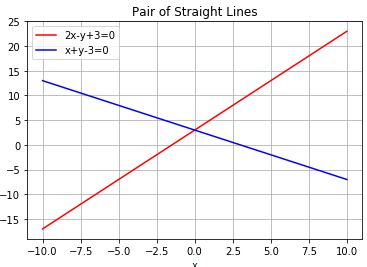
\includegraphics[width=\columnwidth]{./solutions/13/13/Latex/assignment4fig.jpg}
	
	\caption{Pair of Straight Lines}
	
	\label{eq:solutions/13/13/fig:1}
	
\end{figure}

